\section{对偶理论}
\subsection{对偶问题}
对于一个线性规划问题(称为原问题,primal,记为 P)
$$
\max \quad c^Tx
$$
$$
\text{s.t.} 
\begin{cases}
    Ax \le b \\
    x \ge 0
\end{cases}
$$
定义它的对偶问题(dual,记为 D)为
$$
\min \quad b^Ty
$$
$$
\text{s.t.} 
\begin{cases}
    A^Ty \ge c \\
    y \ge 0
\end{cases}
$$
这里的对偶变量 $y$,可以看作是对原问题的每个限制,都用一个变量来表示。 \\~\\
原问题限制条件的不等号,和对偶问题限制条件的不等号,是相互关联的。假设原问题是一个最大化问题,设 $a_i^T$ 表示 $A$ 中的第 $i$ 行,我们有以下结论:
\begin{enumerate}
    \item $a^Tx \_ bx$ 和 $y_i \_ 0$ 关系:
    \begin{table}[!htbp]
        \centering
        \begin{tabular}{|c|c|c|}
            \hline 
            \multicolumn{2}{|c|}{} & $y_i \_ 0$ \\
            \hline
            \multirow{3}*{$a^Tx \_ bx$} & $\le$ & $\ge$ \\
            \cline{2-3}
            & $\ge$ & $\le$ \\
            \cline{2-3}
            & = & 无限制 \\
            \hline
        \end{tabular}
    \end{table}
    \item $x_i \_ 0$ 和 $A^T_iy \_ c_i$ 关系:
    \begin{table}[!htbp]
        \centering
        \begin{tabular}{|c|c|c|}
            \hline 
            \multicolumn{2}{|c|}{} & $A^T_iy \_ c_i$ \\
            \hline
            \multirow{3}*{$x_i \_ 0$} & $\ge$ & $\ge$ \\
            \cline{2-3}
            & $\le$ & $\le$ \\
            \cline{2-3}
            & 无限制 & = \\
            \hline
        \end{tabular}
    \end{table}
\end{enumerate}

\subsection{对偶问题的性质}
\subsubsection{对称性}
对称性 (symmetry),即假设有原问题,以及其对偶问题,则其\textbf{对偶问题的对偶问题即原问题}。 \\
将对偶问题变成标准形式,有
$$
\max \quad y^T(-b)
$$
$$
\text{s.t.} 
\begin{cases}
    (-A^T)y \le -c \\
    y \ge 0
\end{cases}
$$
它的对偶问题是
$$
\min \quad -c^Tx
$$
$$
\text{s.t.} 
\begin{cases}
    -Ax \ge -b \\
    x \ge 0
\end{cases}
$$
把目标函数和限制都乘以 $-1$ 后即原问题。

\subsubsection{弱对偶定理}
弱对偶定理 (weak duality),即假设 $x$ 和 $y$ 分别是原问题和对偶问题的可行解,有 \textbf{$c^Tx \le b^Ty$}。 \\
由 $y$ 的可行性,有 $A^Ty \ge c$,即 $y^TA \ge c^T$,两边同乘以 $x$ ,有 $y^TAx \ge c^Tx$;由 $x$ 的可行性,有 $Ax \le b$,则 $y^TAx \le y^Tb$,合起来就是 $c^Tx \le b^Ty$。

\subsubsection{最优性}
最优性 (optimality),即假设 $x$ 和 $y$ 分别是原问题和对偶问题的可行解,且 $c^Tx = b^Ty$,那么 $x$ 和 $y$ 分别是原问题和对偶问题的最优解。

\subsubsection{无界性}
无界性 (unbounded),即
\begin{enumerate}
    \item 若原问题有可行解无最优解(目标函数值可以取无穷大),则对偶问题无可行解。
    \item 若对偶问题有可行解无最优解,则原问题无可行解。
\end{enumerate}

\subsubsection{强对偶定理}
强对偶定理 (strong duality),即\textbf{若原问题(或对偶问题)有有限最优解,则对偶问题(或原问题)也有有限最优解,且最优解相等}。
以下通过通过单纯形法的计算过程辅助证明: \\~\\~\\
假设加上松弛变量后,原问题变为
$$
\max \quad c^Tx
$$
$$
\text{s.t.} 
\begin{cases}
    \bar{A}x = b \\
    x \ge 0
\end{cases}
$$
有初始单纯形表
$$
\begin{array}{c|cc|c} & c^T & 0 & 0 \\ \hline x^*_B & A & I & b \end{array}
$$
最终单纯形表为
$$
\begin{array}{c|cc|c} & c^T - c^T_B\bar{A}_B^{-1}A & -c^T_B\bar{A}_B^{-1} & -c^T_B\bar{A}_B^{-1}b \\ \hline x^*_B & \bar{A}_B^{-1}A & \bar{A}_B^{-1} & \bar{A}_B^{-1}b \end{array}
$$
由于 $x^*_B$ 是原问题最优的基变量组合,则检验数均非正,有
\begin{align}
& c^T \le c^T_B\bar{A}_B^{-1}A \tag{1} \\
& -c^T_B\bar{A}_B^{-1} \le 0 \tag{2}
\end{align}
取 $y^{*T} = c^T_B\bar{A}_B^{-1}$,代入以上条件$(1)$和$(2)$,有 $A^Ty^* \ge c$ 和 $y^* \ge 0$,即 $y^*$ 是一个可行解。 \\
根据单纯形法,有 $x^*_B = \bar{A}_B^{-1}b$,$x^*_N = 0$,则对偶问题的目标函数值为 $b^Ty^* = y^{*T}b = c^T_B\bar{A}_B^{-1}b = c^T_Bx^*_B = c^Tx^*$,为一对可行的 $x$ 和 $y$,使得原问题和对偶问题的目标函数值相等。 \\
根据弱对偶定理,这两个可行解分别是原问题和对偶问题的最优解。

\subsubsection{互补松弛定理}
互补松弛定理 (complementary slackness),即假设 $x^*$ 与 $y^*$ 分别是原问题和对偶问题的可行解,以下条件等价:
\begin{enumerate}
    \item $x^*$ 和 $y^*$ 分别是原问题和对偶问题的最优解。
    \item $(y^{*T}A - c^T)x^* = 0$ 且 $y^{*T}(Ax^*-b) = 0$。
\end{enumerate}
有以下证明: \\
$1 \Rightarrow 2$: \\
$y^{*T}b = y^{*T}Ax^* = c^Tx^*$,根据弱对偶定理得 $x^*$ 和 $y^*$ 分别是原问题和对偶问题的最优解。 \\
$2 \Rightarrow 1$: \\
根据弱对偶定理的推导,有 $y^{*T}b \ge y^{*T}Ax^* \ge c^Tx^*$。因为 $x^*$ 和 $y^*$ 分别是原问题和对偶问题的最优解,有 $y^{*T}b = c^Tx^*$,则  $y^{*T}b = y^{*T}Ax^* = c^Tx^*$,即$(y^{*T}A - c^T)x^* = 0$ 且 $y^{*T}(Ax^*-b) = 0$。

\subsection{对偶单纯形法}
对单纯形法的停止条件是所有检验数非正($max$ 问题,若是 $min$ 问题所有检验数非负),根据强对偶定理的推导,当所有检验数非正,此时能构造一个对偶问题的可行解,使得原问题和对偶问题的目标函数值相等,则这两目标函数值分别是原问题和对偶问题的最优解。\\ 
即保证原问题可行解的情况下,尝试构造对偶问题的可行解,如果构造成功,则两个目标函数值都是最优解。 \\
相应地,在保证对偶问题可行解($max$ 问题所有检验数非正, 若是 $min$ 问题所有检验数非负)的情况下,尝试构造原始问题的可行解,如果构造成功,则两个目标函数值都是最优解。 \\
这种单纯形法的变型又称为对偶单纯形法 (dual simplex method)。 \\
对于$min$问题,有以下步骤:
\begin{enumerate}
    \item 找到一组基,使得所有检验数非负。
    \item 若单纯形表中 $b$ 的那一列出现负数,因为有 $x \ge 0$ 的限制,当前基不可行,选择负数中 $b$ 的绝对值最大的那一行(设为第 $i$ 行),对应的变量 $x_i$ 作为出基变量(需将该变量从负数变换为 0)。
    \item 假设第 $i$ 行中,$x_j$ 的系数为 $a_j$,检验数为 $d_j$,则在所有 $a_j < 0$ 的变量中,选择 $d_j/a_j$ 绝对值最小的那一列,对应的变量 $x_k$ 作为入基变量,回到 步骤 $2$。如果所有 $a_j \ge 0$,则原问题无可行解。
    \item 若单纯形表中 $b$ 的那一列均非负,即构造出了一个原问题的可行解,算法结束。
\end{enumerate}
假设有以下问题:
$$
\min \quad 9x_1 + 5x_2 + 3x_3
$$
$$
\text{s.t.} 
\begin{cases}
    3x_1 + 2x_2 - 3x_3 \ge 3 \\
    2x_1 + x_3 \ge 5 \\
    x_1, x_2, x_3 \ge 0
\end{cases}
$$
加入松弛变量后,问题转化为
$$
\min \quad 9x_1 + 5x_2 + 3x_3
$$
$$
\text{s.t.} 
\begin{cases}
    3x_1 + 2x_2 - 3x_3 - x_4 = 3 \\
    2x_1 + x_3 - x_5 = 5 \\
    x_1, x_2, x_3, x_4, x_5 \ge 0
\end{cases}
$$
有初始单纯形表
$$
\begin{array}{c|ccccc|c} & 9 & 5 & 3 & 0 & 0 & 0 \\ \hline x_4 & -3 & -2 & 3 & 1 & 0 & -3 \\ x_5 & -2 & 0 & -1 & 0 & 1 & -5 \end{array}
$$
选择 $x_5$ 出基. 由于 $3/1 < 9/2$,选择 $x_3$ 入基,有
$$
\begin{array}{c|ccccc|c} & 3 & 5 & 0 & 0 & 3 & -15 \\ \hline x_4 & -9 & -2 & 0 & 1 & 3 & -18 \\ x_3 & 2 & 0 & 1 & 0 & -1 & 5 \end{array}
$$
选择 $x_4$ 出基. 由于 $3/9 < 5/2$,选择 $x_1$ 入基,有
$$
\begin{array}{c|ccccc|c} & 0 & 13/3 & 0 & 1/3 & 4 & -21 \\ \hline x_1 & 1 & 2/9 & 0 & -1/9 & -1/3 & 2 \\ x_3 & 0 & -4/9 & 1 & 2/9 & -1/3 & 1 \end{array}
$$
此时最后一列第二、三行均非负,迭代结束。原问题的最优解为 $x_1 = 2, x_2 = 0, x_3 = 1$,目标函数值为 $21$。

\subsection{原始对偶方法}
假设已知对偶问题的可行解 $y$ ,需要寻找一个原问题的可行解 $x$ 满足互补松弛定理。
假设 $A_j$ 表示矩阵 $A$ 的第 $j$ 列,定义 $J = \{ j | A_j^Ty = c_j \}$(称 $J$ 为允许指标集)。根据原问题的定义和互补松弛定理,有
\begin{align}
& Ax = b \tag{1} \\ 
& x_j = 0 \quad \forall j \not\in J \tag{2} \\ 
& x_j \ge 0 \quad \forall j \in J \tag{3}
\end{align}
如果能找到一个 $x$ 满足上面三个条件,$x$ 和 $y$ 就能满足互补松弛定理。 \\
为了获得一个可行的 $x$,构造一个优化问题,称为限制的原问题(restricted primal, RP)。
$$
\min \quad \sum_{i = 1}^m \bar{x_i}
$$
$$
\text{s.t.} 
\begin{cases}
    \sum_{j \in J} a_{i, j}x_j + \bar{x_i} = b_i \\
    x_j \ge 0, \bar{x_i} \ge 0
\end{cases}
$$
若目标函数值取 $0$,则得到满足互补松弛定理的 $x$。
写出 RP 的对偶问题,称为限制的对偶问题(dual restricted primal, DRP)。 \\~\\ \pagebreak
$$
\max \quad b^Ty
$$
$$
\text{s.t.} 
\begin{cases}
    A^T_jy \le 0, \ \forall j \in J \\
    y_i \le 1, \ \forall i \in \{1, 2, \ \cdots, m\}
\end{cases}
$$
假设 $\bar{y}$ 为 DRP 的最优解,根据强对偶定理,若 $b^T\bar{y} = 0$ ,则 RP 的目标函数值也可以取 $0$,则当前对偶可行的 $y$ 就是对偶问题的最优解;否则有 $b^T\bar{y} \ge 0$,因为至少 $\bar{y} = 0$ 是 DRP 的可行解。 \\
如果发现 RP 问题无可行解,或者 DRP 问题无有限最优解,则原问题无可行解。 \\~\\
如果 DRP 的最优解让 DRP 的目标函数值超过 $0$,说明当前的 $y$ 还不是最优的。\\ 
假设新的对偶可行解 $\hat{y} = y + \theta\bar{y}$($\theta \ge 0$),有 $b^T\hat{y} = b^Ty + \theta b^T\bar{y} > b^Ty$,改进对偶问题的目标函数值。由于 $\hat{y}$ 仍然是对偶可行的,即必须满足 $A^T\hat{y} = A^Ty + \theta A^T\hat{y} \le c$ 。 \\
对于 $j \in J$,因为 $A^T_j\bar{y} \le 0$,无论 $\theta$ 取多大,都不会超过 $c$ 的限制;对于 $j \not\in J$,选择
$$
\theta = \min_{j \not\in J, A^T_j\bar{y} > 0} \quad \frac{c_j - A^T_jy}{A^T_j\bar{y}}
$$
使得 $j \not\in J$ 中的一条限制变紧,其它限制不会超过,仍然是对偶可行的。若 $\theta$ 可以无限增大,则对偶问题没有有限最优解,原问题无可行解。
将 $y$ 调整为 $\hat{y}$ 之后,进入下一轮迭代继续调整,直到 DRP 的最优解让目标函数值为 $0$,此时的 $y$ 就是对偶问题的最优解。

\subsubsection{应用:最短路问题}
考虑有向图上的最短路问题,起点为 $s$,终点为 $t$。对有向图定义点 - 弧关联矩阵,若一条边是一个顶点的出边,那么矩阵对应元素为 $1$;若一条边是一个顶点的入边,那么矩阵对应元素为 $-1$。假设 $w_i$ 表示第 $i$ 条边的长度,$x_i$ 表示第 $i$ 条边是否在最短路上,
可构造线性规划问题
$$
\min \quad w^Tx
$$
$$
\text{s.t.} 
\begin{cases}
    Ax = v \\
    x \ge 0
\end{cases}
$$
因为 $s$ 为起点,$t$ 为终点,
$$
v_i = \begin{cases} 1 & i = s \\ -1 & i = t \\ 0 & \text{otherwise} \end{cases}
$$
根据点 - 弧关联矩阵的定义很容易发现,把 $A$ 的每一行加起来,最后会获得都是 $0$ 的一行,即 $A$ 中的行向量线性相关。可从 $A$ 中去掉代表终点 $t$ 的那一行,得到新矩阵 $\bar{A}$。 \\
得到新的线性规划问题
$$
\min \quad w^Tx
$$
$$
\text{s.t.} 
\begin{cases}
    \bar{A}x = v \\
    x \ge 0
\end{cases}
$$
其中
$$
v_i = \begin{cases} 1 & i = s \\ 0 & \text{otherwise} \end{cases}
$$
写出对偶问题
$$
\max \quad \pi_s
$$
$$
\text{s.t.} 
\begin{cases}
    \pi_i - \pi_j \le w_e, \ \forall e = (i, j) \in E \\
    \pi_t = 0
\end{cases}
$$
只要令$\pi = 0$ 即可得到对偶问题的可行解。 \\
写出DRP
$$
\max \quad \pi_s
$$
$$
\text{s.t.} 
\begin{cases}
    \pi_i - \pi_j \le 0, \ \forall (i, j) \in J \\
    \pi_i \le 1 \\
    \pi_t = 0
\end{cases}
$$
如果已知从点 $s$ 到某点 $p$ 的最短路,而边 $j$ 就在这条最短路上,根据最短路的三角不等式,这条边一定在 $j$ 中。假设 $C$ 为已知最短路的点构成的连通块,为了让 $\pi_s$ 的取值最大并满足 DRP 的限制条件,$C$ 中所有点的变量值都必须和 $\pi_s$ 相同。若 $t \not\in C$, $\pi_s = 1$;若 $t \in C$,由于 $\pi_t = 0$ 的条件,$\pi_s = 0$,得到了从 $s$ 到 $t$ 的最短路。 \\~\\
假设有以下问题:
\begin{figure}[H]
    \begin{center}
        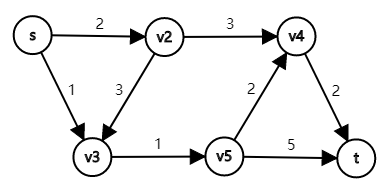
\includegraphics[scale=0.9]{img/drp_shortest_path.png}
        \caption{最短路问题例子。}
    \end{center}
\end{figure}
\begin{table}[!htbp]
    \centering
    \begin{tabular}{c|cccccc} 
        & $\pi_s$ & $\pi_{v_2}$ & $\pi_{v_3}$ & $\pi_{v_4}$ & $\pi_{v_5}$ & $\pi_t$ \\ 
        \hline 
        0 & 0 & 0 & 0 & 0 & 0 & 0 \\ 
        1 & 1 & 0 & 0 & 0 & 0 & 0 \\ 
        2 & 2 & 0 & 1 & 0 & 0 & 0 \\ 
        3 & 4 & 2 & 3 & 0 & 2 & 0 \\ 
        4 & 6 & 5 & 4 & 2 & 4 & 0
    \end{tabular}
    \caption{最短路问题例子迭代过程。}
    \label{table:drp_shortest_path}
\end{table}
绘制表格,记录每次迭代的 $\pi$ 值。通过表\ref{table:drp_shortest_path} ,经过 $4$ 次迭代,得到 $s$ - $t$ 的最短路为 $6$。

\pagebreak
